% Gemini theme
% https://github.com/anishathalye/gemini
%
% We try to keep this Overleaf template in sync with the canonical source on
% GitHub, but it's recommended that you obtain the template directly from
% GitHub to ensure that you are using the latest version.

\documentclass[final,10pt]{beamer}

% ====================
% Packages
% ====================
\usefonttheme{professionalfonts}
\usefonttheme{serif}
\usepackage{ragged2e}
\usepackage[T1]{fontenc}
\usepackage{lmodern}
\usepackage[orientation=portrait,size=a0,scale=1]{beamerposter}
\usetheme{gemini}
\usecolortheme{gemini}
\usepackage{graphicx}
\usepackage{booktabs}
\usepackage{amsmath}
\usepackage{epsfig}
\usepackage{epstopdf}
\usepackage[dvipsnames]{xcolor}
\usepackage{subcaption}
\usepackage{caption}


\usepackage{epsf}
\input{epsf.sty}
\usepackage{graphicx,amsmath,amssymb}
\usepackage{graphicx}
%\usepackage[export]{adjustbox}
\usepackage{epsfig,multicol}
\usepackage{multirow}
\usepackage{amsmath}

\hypersetup{
  colorlinks=true,
  citecolor=magenta,
  linkcolor=blue,
  urlcolor=violet
 }
 \usepackage{tikz}
\usetikzlibrary{arrows.meta}
\usetikzlibrary{angles,quotes} % for pic
\usetikzlibrary{decorations.markings,arrows.meta}
\tikzset{midarr/.style={decoration={markings,mark=at position #1 with {\arrow{stealth}}},postaction={decorate}},
  midarr/.default=0.5 }
\usetikzlibrary{shapes.geometric, arrows}
\usetikzlibrary{shapes,positioning}
\tikzstyle{startstop} = [rectangle, rounded corners, minimum width=2cm, minimum height=1cm,text centered, text width=4.4cm, draw=black, fill=white!30]
\tikzstyle{io} = [trapezium, trapezium left angle=70, trapezium right angle=110, minimum width=2cm, minimum height=1cm, text centered, draw=black]
\tikzstyle{process} = [rectangle, minimum width=1.5cm, minimum height=1cm, text centered,, text width=4cm, draw=black, fill=white!30]
\tikzstyle{decision} = [diamond, minimum width=3cm, minimum height=1cm, text centered, text width=4.2cm, draw=black, fill=green!30]
\tikzstyle{arrow} = [thick,->,>=stealth]

\usepackage[framemethod=TikZ]{mdframed}
\usepackage{lipsum}

\usetikzlibrary{arrows}
\usetikzlibrary{shapes}

\usepackage{stackengine}
\usepackage{pgfplots}
\stackMath
\pgfplotsset{compat=1.14}


% ====================
% Lengths
% ====================

% If you have N columns, choose \sepwidth and \colwidth such that
% (N+1)*\sepwidth + N*\colwidth = \paperwidth
\newlength{\sepwidth}
\newlength{\colwidth}
% \setlength{\sepwidth}{0.025\paperwidth}
% \setlength{\colwidth}{0.3\paperwidth}

\setlength{\sepwidth}{0.033\paperwidth}
\setlength{\colwidth}{0.45\paperwidth}


\newcommand{\separatorcolumn}{\begin{column}{\sepwidth}\end{column}}
\newcommand{\squeezeup}{\vspace{-4mm}}
% ====================
% Title
% ====================

\title{\boldmath Quantum Modular Forms in Knot Theory}

\author{Kabir Bajaj\inst{1}, Rehmat Singh Chawla\inst{1}}
\institute{\inst{1} Department of Physics, Indian Institute of Technology Bombay}


\footercontent{
  \hfill Symphy 2024}
  
% (can be left out to remove footer)

% ====================
% Logo (optional)
% ====================

% use this to include logos on the left and/or right side of the header:
% \logoright{\includegraphics[height=7cm]{logo1.pdf}}
% \logoleft{\includegraphics[height=7cm]{logo2.pdf}}
\newcommand{\mathsym}[1]{{}}
\newcommand{\unicode}[1]{{}}
\newcommand{\tr}{\operatorname{Tr}}
\newcommand{\ad}{\operatorname{ad}}
\newcommand{\vect}[1]{\boldsymbol{#1}}
\newcommand{\R}{\mathbb{R}}
\newcommand{\C}{\mathbb{C}}
\newcommand{\N}{\mathbb{N}}
\newcommand{\Z}{\mathbb{Z}}
\newcommand{\Q}{\mathbb{Q}}
\newcommand{\I}{\mathbb{I}}
\newcommand{\calL}{\mathcal{L}}
% ====================
% Body
% ====================
\begin{document}

\addtobeamertemplate{headline}{}
{
    \begin{tikzpicture}[remember picture,overlay]
      \node [anchor=north west, inner sep=3cm] at ([xshift=106.5cm,yshift=2cm]current page.north west)
      {
\includegraphics[height=8.6cm]{logo.png}};
    \end{tikzpicture}
}
\begin{frame}[t]
\begin{columns}[t]
\separatorcolumn

\begin{column}{\colwidth}


\begin{block}{Motivation}
Knot Theory formalises intuitive notions of knots and links. The central problem in Knot Theory is to characterise and differentiate knots using topological quantities which are invariant for a particular knot but can differ between knots. We explore the connection between knot invariants and curious mathematical objects called Quantum Modular Forms.
\end{block}


\begin{block}{Modular Forms}
    \begin{itemize}
        \item The \textbf{Modular group} $\text{PSL}_2(\Z)=\text{SL}_2(\Z)/\{\pm \I\}$ acts as $\left(\!\begin{smallmatrix}a&b\\c&d\end{smallmatrix}\!\right) z = \frac{az+b}{cz+d}$ on $z\in\C\cup\{\infty\}$.
    
        \item A \textbf{modular form} is a holomorphic function on $H$(upper half complex plane)$\cup\{\infty\}$ transforming as $f(\gamma z)=\epsilon(\gamma)(cz+d)^{2k}f(z)\; \forall \gamma\in\mathrm{PSL}_2(\Z)$,  $|\epsilon(\gamma)| = 1$
    \end{itemize}
\end{block}

\begin{block}{Quantum Modular Forms}
A \textbf{quantum modular form} of weight k ($k \in \mathbb{Z}/2$) is a function $g : \mathbb{Q}/S \rightarrow \mathbb{C}$, for some discrete subset S, such that for all $\gamma = \left(\!\begin{smallmatrix}a&b\\c&d\end{smallmatrix}\!\right) \in \Gamma \subseteq \mathrm{SL}_2, (\mathbb{Z}) $ the functions :
\begin{equation}
    h_{g,\gamma}(x) : = g(x) - \epsilon(\gamma)^{-1}(cx+d)^{-2k}g(\gamma x)
\end{equation}
satisfy a suitable property of continuity or analyticity in $\mathbb{R}$ (definitions vary).
    
\textbf{Examples of QMFs}\vspace*{-0.7em}
\begin{itemize}
    \item  Kontsevich (1997), Zagier (2001), Kashaev (1996):  $F(\zeta_N) : =\sum_{n=0}^{\infty} (\zeta_N)_{n}$, where $(x)_{n} = \prod_{k = 0}^{n-1}(x-k)$ and $(\zeta_N)^N = 1$.
    \item Kashaev (1996): $J(\zeta_N) : = \sum_{n=0}^{\infty} |(\zeta_N)_{n}|^2$.
    \item Lawrence - Zagier (1999): $W(\zeta_K) := \frac{-1-i}{\sqrt{120K}}\sum\limits_{\substack{\beta \mod 60K,\\ \beta \neq 0 \mod K}} \frac{\sin(\frac{\pi \beta}{3K})\sin(\frac{\pi \beta}{5K})}{\cos(\frac{\pi \beta}{2K})}e^{-\pi i (\beta^2+1)/60K} $
\end{itemize}
\end{block}


\begin{block}{Knot Theory}
\begin{itemize}
    \item A \textbf{knot} is a closed path embedded in a 3-manifold, generally $\R^3$.
    \item A \textbf{link} is a collection of knots, possibly intertwined.
    \begin{figure}[!h]
        \centering
        \begin{subfigure}{0.4\textwidth}
            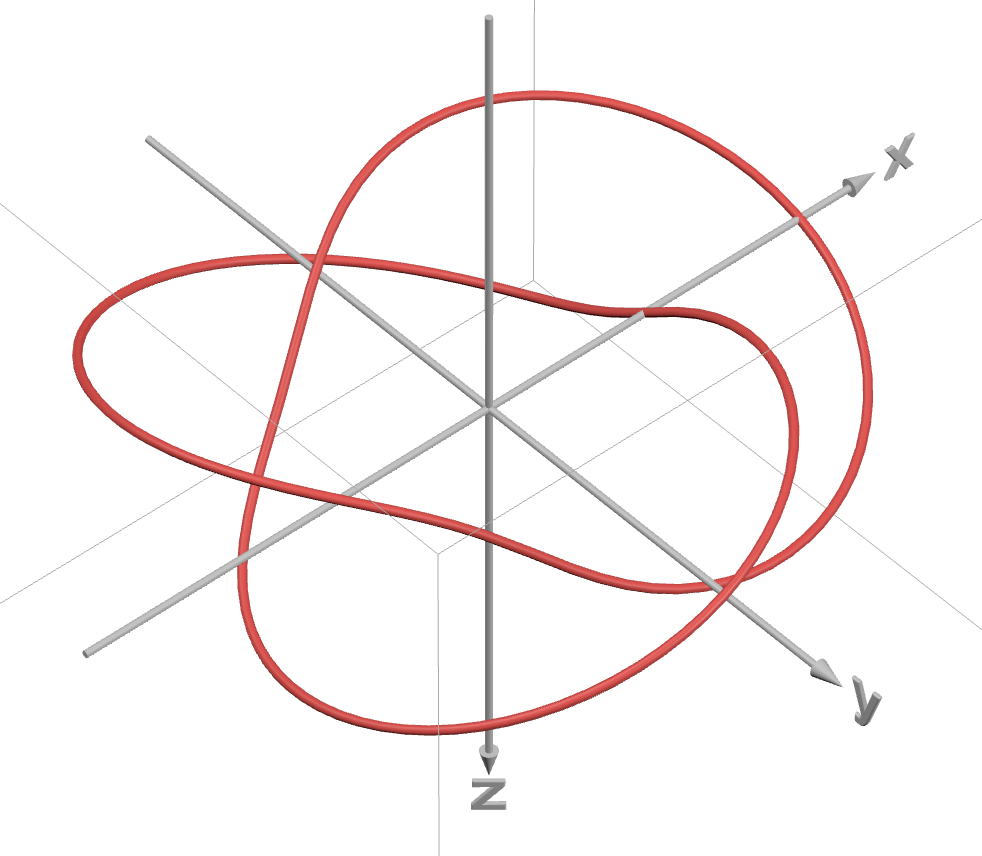
\includegraphics[width=0.8\textwidth]{Figures/trefoil_3d.png}
        \end{subfigure}
        \begin{subfigure}{0.4\textwidth}
            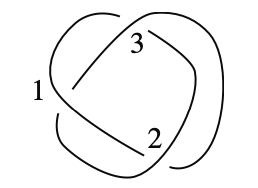
\includegraphics[width=0.8\textwidth]{Figures/Trefoil.png}
        \end{subfigure}
        \caption{The trefoil knot and its 2D diagram with labelled crossings.}
    \end{figure}\vspace*{-0.5em}
    \item A famous knot invariant is the \textbf{Jones Polynomial}, a Laurent polynomial generated via a recursive relation between knots related by the addition of a single crossing.
    \item Witten showed that the Jones polynomial for a knot can be obtained as the expectation value of the corresponding Wilson loop operator in a Chern-Simons field theory with gauge group $SU(2)$.
    \item The \textbf{coloured Jones polynomials} are generalisations obtained from the $SU(N)$ Chern-Simons theories (see below).
    \item \textbf{Torus knots} are knots embedded on the surface of a torus in $\R^3$. The $(p,q)$ torus knot winds $q$ times around the interior of the torus and $p$ times around its axis - the trefoil is the $(2,3)$ torus knot. $(p,q)$ must be coprime.
    They can be parametrised as \begin{gather}
        \left(\cos p\theta(R+r\cos q\theta),\; \sin p\theta(R+r\cos q\theta),\; -r\sin q\theta\right)\\
        \theta\in {[0,2\pi]}\nonumber
    \end{gather}
    % \item The \textbf{Reidmeister moves} are the 3 moves on a knot diagram corresponding to physical movement of the knot - diagrams linked by Reidmeister moves represent the same knot.
\end{itemize}
% \begin{figure}[!h]
%     \centering
%     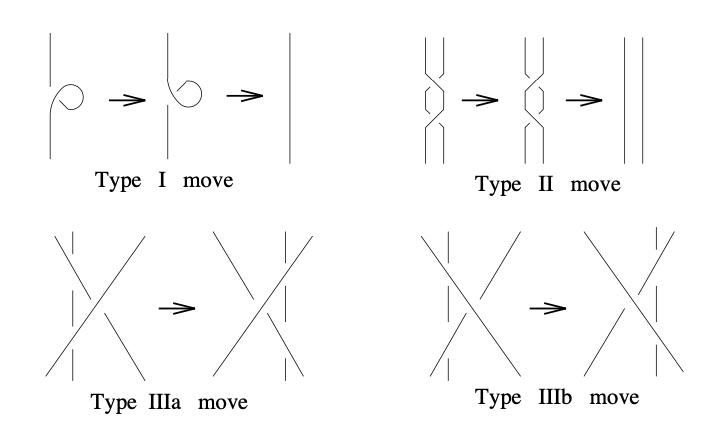
\includegraphics[width=0.8\textwidth]{Figures/Reidmeister.png}
% \end{figure}

\end{block}


\end{column}
\separatorcolumn
\begin{column}{\colwidth}

\begin{block}{Chern-Simons Theory}
    Composed of 
\begin{itemize}
    \item A differentiable, compact 3-manifold $M$
    \item A simple, compact gauge group $G$ (with corresponding gauge connection $A$, a 1-form) 
    \item Integer parameter $k$ (required to be integral for gauge invariance)
\end{itemize}
Then we have a Chern-Simons form, which integrates to give the action:
\begin{equation}
    S_{CS}[A] = \int _M\text{Tr}(A\wedge dA +\frac 23 A\wedge A\wedge A)
\end{equation}
The Wilson loop operator for a knot $K$ is given by an integral over the knot:
\begin{gather}
    W[K] = \exp \left(\iota n_i \oint_{K} dx^\mu A_\mu(x) \right)
\end{gather}
The expectation value of a Wilson loop operator for gauge groups $SU(N)$ give the coloured Jones polynomials in the variable $q=\exp\frac{2\pi\iota}{k+h}$ for the knot $K$.

\end{block}



\begin{block}{Torus Knots and Quantum Modular Forms}
\textbf{Example : Trefoil}

The coloured Jones polynomial can be computed by associating tensorial factor to each crossing and contracting the indices of connected crossings. We write down the result for a trefoil in the fundamental representation of any $SU(N)$:
\begin{equation}
    J_N(T_{2,3},q) = q^{1-N} \sum_{n=0}^\infty q^{-nN}(q^{1-N})_n
\end{equation}
This can be rewritten in the Kontsevich-Zagier series, a well-known Quantum Modular Form we discussed previously.
\begin{equation}
    J_N(T_{2,3},\zeta_N)=\zeta_NF(\zeta_N)
\end{equation}

\textbf{$T_{(2,2t+1)}$ Torus Knots}
\begin{gather}
    J_N(T_{(s,t)},\zeta_N) = \zeta_N^{\frac{s^2t^2-s^2-t^2}{4st}} \tilde\Phi_{s,t}^{s-1,1}(\tfrac 1 N)\\
    \tilde\Phi_{s,t}^{n,m}(\tau) := -\frac 12 \sum\limits_{k=0}^\infty k \chi_{s,t}^{n,m}(k) \exp\frac{2\pi \iota\tau  k^2}{4st}\\
    \chi_{s,t}^{n,m}(k) := \begin{cases}
        1 & k=\pm(nt-ms)\mod 2st\\
    -1 & k = \pm (nt+ms) \mod 2st\\
0 & \text{otherwise} \end{cases}
\end{gather}

\end{block}

\end{column}

\separatorcolumn


\end{columns}
\end{frame}


\end{document}
